\documentclass[
	12pt,				% tamanho da fonte
	openright,			% capítulos começam em pág ímpar (insere página vazia caso preciso)
	oneside,			% Impressão de um lado
	a4paper,			% tamanho do papel. 
	english,			% idioma adicional para hifenização
	french,				% idioma adicional para hifenização
	spanish,			% idioma adicional para hifenização
	brazil,sumario=tradicional				% o último idioma é o principal do documento
	]{UFPE-DCP} %Modelo criado a partir do abntex2
	
%%%% Pacotes básicos 
\usepackage{epigraph} % Utilização de epígrafes no começo dos capítulos
%\renewcommand{\epigraphrule}{0pt} % Linha da epígrafe
%Configuração da epígrafe e justificação
\makeatletter
\newlength\interepigraphskip
\setlength\interepigraphskip{0ex}
\renewcommand\epigraph[3][\interepigraphskip]{\vspace{\beforeepigraphskip}
  {\epigraphsize\begin{\epigraphflush}\begin{minipage}{\epigraphwidth}
    \@epitext{#2}\\[#1] \@episource{#3}
    \end{minipage}\end{\epigraphflush}
    \vspace{\afterepigraphskip}}}
\makeatother

\usepackage{type1cm} % retira as restrições de fontes escaláveis
\usepackage{enumerate} % criação de marcadores (numeração)
\usepackage{enumitem} %customizar itens para numeração
\usepackage{multirow} % mesclar linhas e colunas no ambiente tabular
\usepackage{hhline}  % Linhas horizontais para tabela
\usepackage{lastpage}			% Usado pela Ficha catalográfica
\usepackage{indentfirst}		% Indenta o primeiro parágrafo de cada seção.
\usepackage{color}				% Controle das cores
\usepackage[pdftex]{graphicx}		% Inclusão de gráficos 
\usepackage{titletoc}
\usepackage{eso-pic}
\usepackage{microtype} 			% para melhorias de justificação
\usepackage{mathtools} % Alinhar as fórmulas
\usepackage{hyperref} %referências como links
\usepackage{pdfpages}
\usepackage{csquotes} %utilizar caracteres especiais no bibtex
\usepackage{tablefootnote} %notas de rodapé nas tabelas
\usepackage{placeins}
\usepackage{ifxetex}
\ifxetex
  \usepackage{fontspec}
  \defaultfontfeatures{Ligatures={TeX}}
  \setmainfont{Times New Roman}
  \else
\usepackage{newtxtext,newtxmath} %Usar uma fonte similar à times, neste caso new times.
\usepackage[T1]{fontenc}		% Selecao de codigos de fonte.
\usepackage[utf8]{inputenc}		% Codificacao do documento (conversão automática dos acentos)
\fi

\renewcommand{\ABNTEXchapterfont}{\normalfont}


% ---
% Pacotes adicionais, usados apenas no âmbito do Modelo Canônico do abnteX2
\renewcommand{\anexoname}{Anexo} % mudar nome do anexo
% ---
\usepackage{lipsum}				% para geração de dummy text
% ---

%
% Pacotes adicionais - 
%\usepackage{lscape} %mudar a orientação da página
\usepackage{pdflscape}
\usepackage{trivfloat}  % Criar ambientes e objetos para as listas
\trivfloat{quadro}  %Cria quadros
\trivfloat{grafico} %Cria gráficos
% --- Definir margens
\usepackage[left=3cm,right=2cm,top=3cm,bottom=2cm]{geometry} %magens
%Margens travadas
\setlrmarginsandblock{3cm}{2cm}{*}
\setulmarginsandblock{3cm}{2cm}{*}
\checkandfixthelayout
% Pacotes de citações
\usepackage[alf,abnt-emphasize=bf,abnt-repeated-author-omit=yes,abnt-full-initials=yes]{abntex2cite}	% Citações padrão ABNT
% --- 
% CONFIGURAÇÕES DE PACOTES
% --- 
%Configuração de captions
\usepackage{caption} % fonte das captions, lembre-se da sobreposição dos pacotes.
\usepackage[font=small]{caption} % fonte das captions, lembre-se da sobreposição dos pacotes.
\captionsetup[table]{aboveskip=1.5pt} % espaçamento do caption para a tabela
\captionsetup[grafico]{aboveskip=1.5pt} % espaçamento do caption para a gráfico
\captionsetup[quadro]{aboveskip=1.5pt} % espaçamento do caption para  quadro
\captionsetup[figure]{aboveskip=1.5pt} % espaçamento do caption para  figuras
\captionsetup[tabular]{aboveskip=1.5pt} % espaçamento do caption para  figuras
% Identação dos Footnotes
\usepackage[hang]{footmisc}
\renewcommand{\hangfootparindent}{2em}% Indentation for 2nd etc. paragraphs in footnotes which cosists of more than one paragraph
\renewcommand{\hangfootparskip}{3pt}% Vertical space between paragraphs in multiparagraph footnotes
\renewcommand{\footnotemargin}{0.00001pt}% Setting left margin; this is the smallest value I can get to have second etc. lines indented to footnote number; zero put indentation to some positive value, and negative values do not help actually
\renewcommand{\footnotelayout}{\hspace{1.0em}}% Here you can modify the spacing between the footnote number and the text of footnote; keep this value and \hangfootparindent value the same
\setlength{\skip\footins}{1cm} % Distâncai das notas para o texto - o famoso filete
\counterwithout{footnote}{chapter} % notas de rodapés com numeração contínua 
\renewcommand\footnoterule{\rule{\linewidth}{0pt}} % espessura e tamanho da linha da nota de rodapé 
% ---Estilo dos capítulos
\makeatletter
\newcommand\thickhrulefill{\leavevmode \leaders \hrule height 1ex \hfill \kern \z@}
\setlength\midchapskip{10pt}
\makechapterstyle{VZ14}{
\renewcommand\chapternamenum{}
\renewcommand\printchaptername{}
\renewcommand\chapnamefont{\bfseries\huge\scshape}
\renewcommand\printchapternum{%
\chapnamefont\null\thickhrulefill\quad
\@chapapp\space\thechapter\quad\thickhrulefill}
\renewcommand\printchapternonum{%
\par\thickhrulefill\par\vskip\midchapskip
\hrule\vskip\midchapskip
}
\renewcommand\chaptitlefont{\Huge\scshape\centering}
\renewcommand\afterchapternum{%
\par\nobreak\vskip\midchapskip\hrule\vskip\midchapskip}
\renewcommand\afterchaptertitle{%
\par\vskip\midchapskip\hrule\nobreak\vskip\afterchapskip}
  \setlength\midchapskip{1pt} % Retirar o box preto
        \renewcommand*{\afterchapternum}{\par\nobreak\vskip 3pt} %Distância do título 1 para o título 2



}
\makeatother
\chapterstyle{VZ14}
   \setlength{\afterchapskip}{50pt} %distância do título do capítulo para o parágrafo
\renewcommand{\chapterheadstart}{\vspace*{-3.52\baselineskip}} % separação superior
%%%
\usepackage{titlesec}
\titleformat{\section}
  {\normalfont\scshape\bfseries\Large}{\thesection}{1em}{}[\vspace{0.2ex}\titlerule]
  
  \titleformat{\subsection}
  {\normalfont\scshape\bfseries\large}{\thesubsection}{1em}{}
  
    \titleformat{\subsubsection}
  {\normalfont\scshape\bfseries\normalsize}{\thesubsubsection}{1em}{}
 % Fim da customização do estilo do chapter



% --- Centralizar valores de quadros nas linhas
\usepackage{array}
\newcolumntype{P}[1]{>{\centering\arraybackslash}p{#1}} %criar paragráfo centralizado "P" maiúsculo
% ---
% Informações de dados para CAPA e FOLHA DE ROSTO
% ---

\titulo{\normalfont\textbf{ MODELO: ELABORAÇÃO DE TRABALHO CIENTÍFICO}}
\autor{\normalfont Fulano Beltrano de Tal}
\local{\normalfont \textit{Dreamland}}
\data{2019}
\orientador[Orientadora:]{Profa. Dra. Sicrana} %Se o orientador for homem retire os colchetes para voltar ao normal.
%\coorientador[Coorientadora:]{Fulano}  % Se possuir coorientador retire o símbolo de porcentagem

\tipotrabalho{Dissertação (Mestrado)}
\preambulo{Dissertação apresentada ao Programa de Pós-graduação em Ciências do Departamento de Ciências da Universidade Federal de Sei  das Quantas, como requisito para obtenção do título de mestre em Ciências.}

% Configurações de aparência do PDF final

% alterando o aspecto da cor azul
\definecolor{blue}{RGB}{41,5,195}

% informações do PDF
\makeatletter
\hypersetup{
     	%pagebackref=true,
		pdftitle={\@title}, 
		pdfauthor={\@author},
    	pdfsubject={\imprimirpreambulo},
	    pdfcreator={\@author},
		pdfkeywords={Palavra-chave 1}{Palavra-chave 2}{Palavra-chave 3}{Palavra-chave 4}{Palavra-chave 5}, 
		colorlinks=true,       		% false: boxed links; true: colored links
    	linkcolor=black,          	% color of internal links
    	citecolor=black,        		% color of links to bibliography
    	filecolor=blue,      		% color of file links
		urlcolor=blue,
		bookmarksdepth=4
} 

\addto\captionsbrazil{
	%\renewcommand{\bibname}{\uppercase{REFER\^ENCIAS}}
}
\makeatother
% --- 
\newcommand{\anexoautorefname}{\normalfont\textbf{Anexo}} % Criação do nome anexo
\newcommand{\nomeanexo}{\normalfont\textbf{Anexo}}
\renewcommand{\bibname}{Referências}    % Renovação do nome das referências
    
% --- 
% Espaçamentos entre linhas e parágrafos 
% --- 
\usepackage{setspace}  % Pacote para controlar espaçamentos 

% O tamanho do parágrafo é dado por:
\setlength{\parindent}{1.3cm}

% Controle do espaçamento entre um parágrafo e outro:
\setlength{\parskip}{0cm}  % tente também \onelineskip

% ---
% compila o indice
% ---
\makeindex
% ---
\usepackage{etoolbox}
\preto\section{%
  \ifnum\value{section}=0\addtocontents{lof}{\vskip10pt}\fi
}

\preto\section{%
  \ifnum\value{section}=0\addtocontents{lot}{\vskip10pt}\fi
}


% Configurando estilos de páginas
%Estilo para página do capítulo
\usepackage{fancyhdr} % Pacote para criação estilos de páginas específicas 
\fancypagestyle{capitulo}{
\fancyhead{}
\fancyfoot{}
\lhead{}
\rhead{}
\rfoot{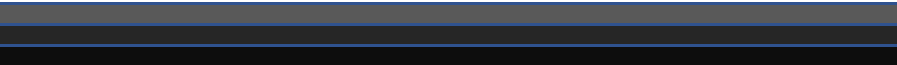
\includegraphics[width=16cm,height=0.4cm]{marca_alta.pdf}}  % Esse comando cria um painel no rodapé. Uma linha ou qualquer figura que queira utilizar
\renewcommand{\headrulewidth}{0pt}
\renewcommand{\footrulewidth}{0pt}
}


%\rhead{ \fbox{$\mu$}\textcircled{$\mu$}}   % comando para utilizar símbolos no canto direito do cabeçalho
\renewcommand{\chaptermark}[1]{\markboth{#1}{}}
\renewcommand{\sectionmark}[1]{\markright{#1}{}}
%Estilo para página do texto
\fancypagestyle{texto}{
\fancyhf{}
\rhead{Página \fbox{\thepage}}
\lhead{\textit{\chaptername  \thechapter : \leftmark}}
\chead{ }
\rfoot{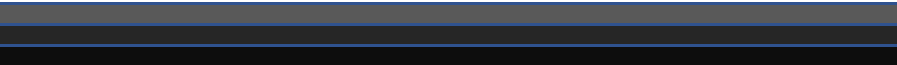
\includegraphics[width=16cm,height=0.4cm]{marca_alta.pdf}}
\lfoot{ }
\cfoot{ }
\renewcommand{\headrulewidth}{0.4pt}
\renewcommand{\footrulewidth}{0pt}
 

}

\fancypagestyle{introducao}{
\fancyhf{}
\rhead{Página \fbox{\thepage}}
\lhead{\textit{\leftmark}}
\chead{ }
\rfoot{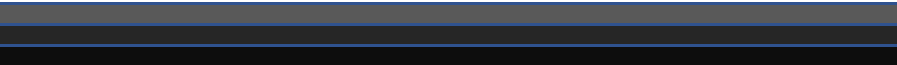
\includegraphics[width=16cm,height=0.4cm]{marca_alta.pdf}}
\lfoot{ }
\cfoot{ }
\renewcommand{\headrulewidth}{0.4pt}
\renewcommand{\footrulewidth}{0pt}
 

}
%Estilo para página das referências
\fancypagestyle{referencias}{
\fancyhf{}
\rhead{Página \fbox{\thepage}}
\lhead{\textit{Referências}}
\chead{ }
\rfoot{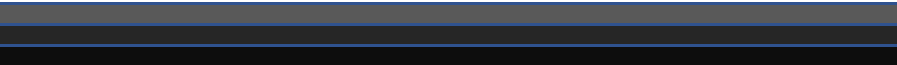
\includegraphics[width=16cm,height=0.4cm]{marca_alta.pdf}}
\lfoot{ }
\cfoot{ }
\renewcommand{\headrulewidth}{0.4pt}
\renewcommand{\footrulewidth}{0pt}
}

\usepackage{afterpage}
\usepackage{nopageno}
% Início do documento
% ----

\begin{document}
% ========= ESSA OPÇÃO É PARA CRIAR A CAPA NORMAL SEM O FUNDO PRETO ====  %

%\begin{figure}[h] 
%\centering % para centralizarmos a figura
%
\includegraphics[width=3cm]{Figuras/ufpelogo.jpg} % leia abaixo
%\end{figure}
%\begin{minipage}{12cm}
%\centering
% \normalfont  Universidade Federal de Sei  das Quantas\\
% \normalfont  Departamento de Ciências\\
% \normalfont  Fulano Beltrano de Tal\\
% \normalfont  Programa de pós-graduação em Ciências\\
%end{minipage}
%\vspace{1cm}
% Seleciona o idioma do documento (conforme pacotes do babel)
%\selectlanguage{english} %caso queira escrever em inglês
\selectlanguage{brazil}
% ========= LEMBRE-SE DE DESATIVAR  A CAPA PRETA NOARQUIVO "UFPE-DCP " NA PASTA DO MODELO    ======= %
% Retira espaço extra obsoleto entre as frases.
\frenchspacing 

% ----------------------------------------------------------
% ELEMENTOS PRÉ-TEXTUAIS
% ----------------------------------------------------------
\pretextual

% ---
% Capa

% ---
\imprimircapa
% ---
\bookmark[dest=TitlePage]{Capa}
% ---
% Folha de rosto
% (o * indica que haverá a ficha bibliográfica)
% ---
\imprimirfolhaderosto*
% ---

% ---
% Inserir a ficha bibliografica
% ---

% Isto é um exemplo de Ficha Catalográfica, ou ``Dados internacionais de
% catalogação-na-publicação''. Você pode utilizar este modelo como referência. 
% Porém, provavelmente a biblioteca da sua universidade lhe fornecerá um PDF
% com a ficha catalográfica definitiva após a defesa do trabalho. Quando estiver
% com o documento, salve-o como PDF no diretório do seu projeto e substitua todo
% o conteúdo de implementação deste arquivo pelo comando abaixo:
%
%\begin{fichacatalografica}
%     \includepdf{ficha-catalografica.pdf}
% \end{fichacatalografica}

\begin{fichacatalografica}
	\sffamily
	\vspace*{\fill}					% Posição vertical
	\begin{center}					% Minipage Centralizado
	\fbox{\begin{minipage}[c][8cm]{13.5cm}		% Largura
	\small
	\imprimirautor
	%Sobrenome, Nome do autor
	
	\hspace{0.5cm} \imprimirtitulo  / \imprimirautor. --
	\imprimirlocal, \imprimirdata-
	
	\hspace{0.5cm} \pageref{LastPage} p. : il. (algumas color.) ; 30 cm.\\
	
	\hspace{0.5cm} \imprimirorientadorRotulo~\imprimirorientador\\
	
\hspace{0.5cm}
	\parbox[t]{\textwidth}{\imprimirtipotrabalho~--~\imprimirinstituicao,
	\imprimirdata.}\\
	
	\hspace{0.5cm}
		1. Palavra-chave1.
		2. Palavra-chave2.
		2. Palavra-chave3.
		I. Orientador.
		II. Universidade xxx.
		III. Faculdade de xxx.
		IV. Título 			
\end{minipage}}
	\end{center}
\end{fichacatalografica}
% ---

% ---
% Inserir errata
% ---
\begin{errata}
%Elemento opcional da \citeonline[4.2.1.2]{NBR14724:2011}. Exemplo:

\vspace{\onelineskip}

Exemplo: FERRIGNO, C. R. A. \textbf{Tratamento de neoplasias ósseas apendiculares com
reimplantação de enxerto ósseo autólogo autoclavado associado ao plasma
rico em plaquetas}: estudo crítico na cirurgia de preservação de membro em
cães. 2011. 128 f. Tese (Livre-Docência) - Faculdade de Medicina Veterinária e
Zootecnia, Universidade de São Paulo, São Paulo, 2011.

\begin{table}[htb]
\center
\footnotesize
\begin{tabular}{|p{1.4cm}|p{1cm}|p{3cm}|p{3cm}|}
 \hline
   \textbf{Folha} & \textbf{Linha}  & \textbf{Onde se lê}  & \textbf{Leia-se}  \\
    \hline
    1 & 10 & auto-conclavo & autoconclavo\\
   \hline
\end{tabular}
\end{table}

\end{errata}
% ---

% ---
% Inserir folha de aprovação
% ---

% Isto é um exemplo de Folha de aprovação, elemento obrigatório da NBR
% 14724/2011 (seção 4.2.1.3). Você pode utilizar este modelo até a aprovação
% do trabalho. Após isso, substitua todo o conteúdo deste arquivo por uma
% imagem da página assinada pela banca com o comando abaixo:
%
% \includepdf{folhadeaprovacao_final.pdf}
%
\begin{folhadeaprovacao}

  \begin{center}
    {\ABNTEXchapterfont\large\imprimirautor}

    \vspace*{\fill}\vspace*{\fill}
    \begin{center}
      \ABNTEXchapterfont\bfseries\Large\imprimirtitulo
    \end{center}
    \vspace*{\fill}
    
    \hspace{.45\textwidth}
    \begin{minipage}{.5\textwidth}
        \imprimirpreambulo
    \end{minipage}%
    \vspace*{\fill}
   \end{center}
        
 Trabalho aprovado. \imprimirlocal, 25 de Abril de 2019:

   \assinatura{\textbf{\imprimirorientador} \\ Orientadora} 
   \assinatura{\textbf{Prof. Beltrano de Sousa} \\ Examinador interno}
   \assinatura{\textbf{Profa. Dra. Fulana da Silva } \\ Examinadora externa}
   %\assinatura{\textbf{Professor} \\ Convidado 3}
   %\assinatura{\textbf{Professor} \\ Convidado 4}
      
   \begin{center}
    \vspace*{0.5cm}
    {\large\imprimirlocal}
    \par
    {\large\imprimirdata}
    \vspace*{1cm}
  \end{center}
  
\end{folhadeaprovacao}

% ---
% Dedicatória
% ---

\begin{dedicatoria}
   \vspace*{\fill}
   \centering
  \noindent
  \textit{Dedicado à todas as pessoas ;)} \vspace*{\fill}
\end{dedicatoria}

% ---
% Agradecimentos
% ---
\begin{agradecimentos}

Agradeço a todos também.

\end{agradecimentos}
% ---

% ---
% Epígrafe
% ---
\begin{epigrafe}
    \vspace*{\fill}
	\begin{flushright}
		\textit{``Coloque uma frase de efeito e que se relacione com o seu tema. Dica de ouro!''\\
		(Autor da citação, pode-se colocar livro e mais informações)}
	\end{flushright}
\end{epigrafe}
% ---

% ---
% RESUMOS
% ---

% resumo em português
\setlength{\absparsep}{18pt} % ajusta o espaçamento dos parágrafos do resumo
\begin{resumo}

 \vspace{\onelineskip}
 
   \noindent 
 \textbf{Palavras-chave}: Palavra-Chave 1. Palavra-Chave 2. Palavra-Chave 3. Palavra-Chave 4. Palavra-Chave 5.% Palavras-chave podem ser separadas por "." ";" "-" ai fica a seu critério e do estabelecimetno de ensino. O ideal é consultar a norma técnica.
\end{resumo}

% resumo em inglês
\begin{resumo}[Abstract]
 \begin{otherlanguage*}{english}
 




   \vspace{\onelineskip}
 
   \noindent 
   \textbf{Keywords}: \textit{keyword 1}. \textit{keyword 2}. \textit{keyword 3}.\textit{ keyword 4}. \textit{keyword 5}.
 \end{otherlanguage*}
\end{resumo}
% ---------
% inserir lista de ilustrações
% ---
\renewcommand{\listfigurename}{Lista de \uppercase{f}iguras}
\pdfbookmark[0]{\listfigurename}{lof}
\listoffigures*
\cleardoublepage
% ---
%LISTA DE GRÁFICOS
% configurações para atender às regras da ABNT
\counterwithout{grafico}{chapter}
\renewcommand{\graficoname}{Gráfico}
\renewcommand{\cftgraficoname}{\graficoname\space } 
\renewcommand{\listgraficoname}{Lista de \uppercase{g}ráficos}
\renewcommand*{\cftgraficoaftersnum}{\hfill--\hfill}
\pdfbookmark[0]{\listgraficoname}{logr}
\listofgraficos*
\cleardoublepage


%-----
%  Lista de Quadros
%---------------
% configurações para atender às regras da ABNT
\counterwithout{quadro}{chapter}
\renewcommand{\cftquadroname}{\quadroname\space } 
\renewcommand{\listquadroname}{Lista de \uppercase{q}uadros}
\renewcommand*{\cftquadroaftersnum}{\hfill--\hfill}
\pdfbookmark[0]{\listquadroname}{loqr}
\listofquadros*


\cleardoublepage
% ---
% inserir lista de tabelas
% ---
\pdfbookmark[0]{\listtablename}{lot}
\renewcommand{\listtablename}{Lista de \uppercase{t}abelas}
\listoftables*
\cleardoublepage
% ---
% inserir o sumario
% --- O COMANDO ABAIXO CRIA UM FUNDO PARA O SUMÁRIO, PARA DESATIVÁ-LO COLOQUE "%" NO COMEÇO DE CADA LINHA 
\AddToShipoutPictureBG*{%
  \AtPageLowerLeft{%
    % Your background image here
    
\includegraphics[width=\paperwidth,height=\paperheight]{toc.pdf}%
  }%
}%
% ATÉ AQUI É O COMANDO PARA PANO DE FUNDO DO SUMÁRIO
\pdfbookmark[0]{\contentsname}{toc}
\tableofcontents*
\cleardoublepage
% ---



% ----------------------------------------------------------
% ELEMENTOS TEXTUAIS
% ----------------------------------------------------------
\textual
% ----------------------------------------------------------
% Introdução (exemplo de capítulo sem numeração, mas presente no Sumário)
% ----------------------------------------------------------
\chapter*[Introdução]{Introdução}
\addcontentsline{toc}{chapter}{Introdução}
\thispagestyle{capitulo}
\lipsum[31]

\lipsum[31]
\lipsum[31]

\lipsum[31]
\lipsum[31]

\lipsum[31]

\newpage
\lipsum[31]
\pagestyle{introducao} % Estilo de página criado especial para a introdução
\lipsum[31]
\cite{talbot2012}
\cite{abntex2modelo}
\cite{abntex2modelo}
\cite{araujo2012}
\cite{memoir}
\cite{abntex2cite}
\cite{abntex2classe}
\cite{NBR10520:2002}
\cite{van86}
\cite{van86}


\cite{ibge1993}
\lipsum[31]
\cite{guizzardi2005}
\cite{macedo2005}
\cite{EIA649B}
	\cite{masolo2010}
	\cite{guarino1995}
	\cite{bates2010}
	\cite{doxiadis1965}
\lipsum[31]

\lipsum[31]

\lipsum[31]


\lipsum[31]

\lipsum[31]


\lipsum[31]

\lipsum[31]


\lipsum[31]

\lipsum[31]


\lipsum[31]

\lipsum[31]


\lipsum[31]

\lipsum[31]


\lipsum[31]

\lipsum[31]


\lipsum[31]

\lipsum[31]


\lipsum[31]

\lipsum[31]


\lipsum[31]

\lipsum[31]


%------
% Fim da introdução
% ------
% ----------------------------------------------------------
% PARTE 1
% ----------------------------------------------------------
%\part{Parte 1}
% --------------------------------------------- 
% Comando para caso queira dividir o trabalho em partes

\chapter{Primeiro Capítulo}

% COMANDO DA EPÍGRAFE ABAIXO - ELEMENTO OPCIONAL
%\epigraph{\textit{\footnotesize	 ``Afirmo muitas vezes que, se você medir aquilo de que está falando e expressar em números, você conhece alguma coisa sobre o assunto; mas, quando você não o pode exprimir em números, seu conhecimento é pobre e insatisfatório.''}}{\scriptsize William Thompson (Lord Kelvin)}
%\thispagestyle{capitulo}
%\hfill \break \par % Uma quebra de linha e mais um parágrafo. Essa opção é viável quando a epígrafe for ativada.



\OnehalfSpacing % espaçamento 1,5 cm.  %SingleSpacing é 1cm. E pode ser controlado com o comando \begin{Spacing}{hfactori} ... \end{Spacing}
Miguel é um exemplo de pessoa bondosa e blá blá blá exemple \lipsum[2]
\lipsum[31]

\lipsum[31]

\lipsum[31]

\lipsum[31]

\lipsum[31]
\pagestyle{texto}
\lipsum[31]

\lipsum[31]\footnote{lipsum[31]}

\lipsum[31]

\lipsum[31]
\section{Primeira Seção} 

\lipsum[31]

\lipsum[31]

\lipsum[31]

\lipsum[31]

\lipsum[31]

\subsection{Primeira Subseção}

\lipsum[31]

\lipsum[31]

\lipsum[31]

\lipsum[31]

\lipsum[31]

\lipsum[31]
\subsubsection{ Primeira Subsubseção}

\lipsum[31]

\lipsum[31]

\lipsum[31]

% ----------------------------------------------------------
% ELEMENTOS PÓS-TEXTUAIS
% ----------------------------------------------------------

\postextual
% ----------------------------------------------------------
\pagestyle{texto}

% ----------------------------------------------------------
% Referências bibliográficas
% ----------------------------------------------------------
 \bibliography{bibliografia} % this is mybib 
\pagestyle{referencias}
%\renewcommand{\thebibliography}{\addcontentsline{toc}{chapter}{\bibname}}{\thepage}
 % \renewcommand{\thepage}{\arabic{page}}\setcounter{page}{\thepage}

% ----------------------------------------------------------
% Glossário
% ----------------------------------------------------------
%
% Consulte o manual da classe abntex2 para orientações sobre o glossário.
%
%\glossary

% ----------------------------------------------------------
% Apêndices
% ----------------------------------------------------------

% ---
% Inicia os apêndices
% ---
%\begin{apendicesenv}

% Imprime uma página indicando o início dos apêndices
%\partapendices

% ----------------------------------------------------------
%\chapter{Quisque libero justo}
% ----------------------------------------------------------

%\lipsum[50]

% ----------------------------------------------------------
%\chapter{Nullam elementum urna vel imperdiet sodales elit ipsum pharetra ligula
%ac pretium ante justo a nulla curabitur tristique arcu eu metus}
% ----------------------------------------------------------
%\lipsum[55-57]

%\end{apendicesenv}
% ---


% ----------------------------------------------------------
% Anexos
% ----------------------------------------------------------

% ---
% Inicia os anexos
% ---
%\begin{anexosenv}

% Imprime uma página indicando o início dos anexos
%\partanexos

% ---
%\chapter{Morbi ultrices rutrum lorem.}
% ---
%\lipsum[30]

% ---
%\chapter{Cras non urna sed feugiat cum sociis natoque penatibus et magnis dis
%parturient montes nascetur ridiculus mus}
% ---

%\lipsum[31]

% ---
%\chapter{Fusce facilisis lacinia dui}
% ---

%\lipsum[32]

%\end{anexosenv}

%---------------------------------------------------------------------
% INDICE REMISSIVO
%---------------------------------------------------------------------
\phantompart
\printindex
%---------------------------------------------------------------------


\end{document}
